\documentclass[landscape]{icsislides}

\usepackage[dvips]{graphicx}
%\usepackage[dvips]{color}
%\usepackage{subfigure}
\usepackage[T1]{fontenc}
\usepackage{psfrag}
\usepackage{xspace}
\usepackage{alltt}
\usepackage{colordvi}

\newcommand{\etc}{\emph{etc.}\xspace}
\newcommand{\ie}{\emph{i.e.,}\xspace}
\newcommand{\eg}{\emph{e.g.,}\xspace}

%\def\makeslidenum#1{\Gray{\fontseries{u}\selectfont#1}}%

%% XXX: comment-out to include logo
\newlogo{}

\begin{document}

%%======================================================================
\begin{titlepage}

\begin{center}
{\LARGE \Red{PIM-SM: Protocol Overview and Xorp Design}} \\
\vskip20pt

\vskip100pt
\begin{tabular}{c}
Pavlin Radoslavov \\
\Gray{International Computer Science Institute}
\end{tabular}

\vskip10pt
\small{August 2003}
\end{center}

\end{titlepage}

% %%======================================================================
% \begin{titlepage}

% \begin{center}
% {\LARGE \bf Xorp}
% \end{center}
% \vspace*{1.0in}
% \begin{center}
% Pavlin Radoslavov\\
% \vspace*{0.5in}
% \small {\it pavlin@icsi.berkeley.edu}\\
% \small International Computer Science Institute\\
% \small Berkeley, CA, USA
% \end{center}

% \end{titlepage}

%%======================================================================
\begin{slide}
\slidetitle{Outline}

\begin{enumerate}
  \item PIM-SM Introduction
  \item PIM-SM Xorp Design
  \item Dependency Tracking Mechanism
  \item Current Status
\end{enumerate}

\end{slide}

%%======================================================================
\begin{slide}
\slidetitle{PIM-SM Introduction}

\begin{itemize}
  \item Brief (truncated) history:
  \begin{itemize}
    \item Sigcomm 1994 paper
    \item I-D (PIM-SMv1) and Cisco implementation
    \item June 1997: First experimental RFC-2117 (PIM-SMv2: not compatible
    with v1)
    \item June 1998: Second experimental RFC-2362
    \item July 2003: a new spec (rewritten from scratch, much more
  ``implementor-friendly'') almost ready for RFC publication
  \end{itemize}

  \item Fairly complicated protocol: 104+27 (or 138+35) pages

\end{itemize}

\end{slide}

%%======================================================================
\begin{slide}
\slidetitle{PIM-SM Example}

\begin{center}
  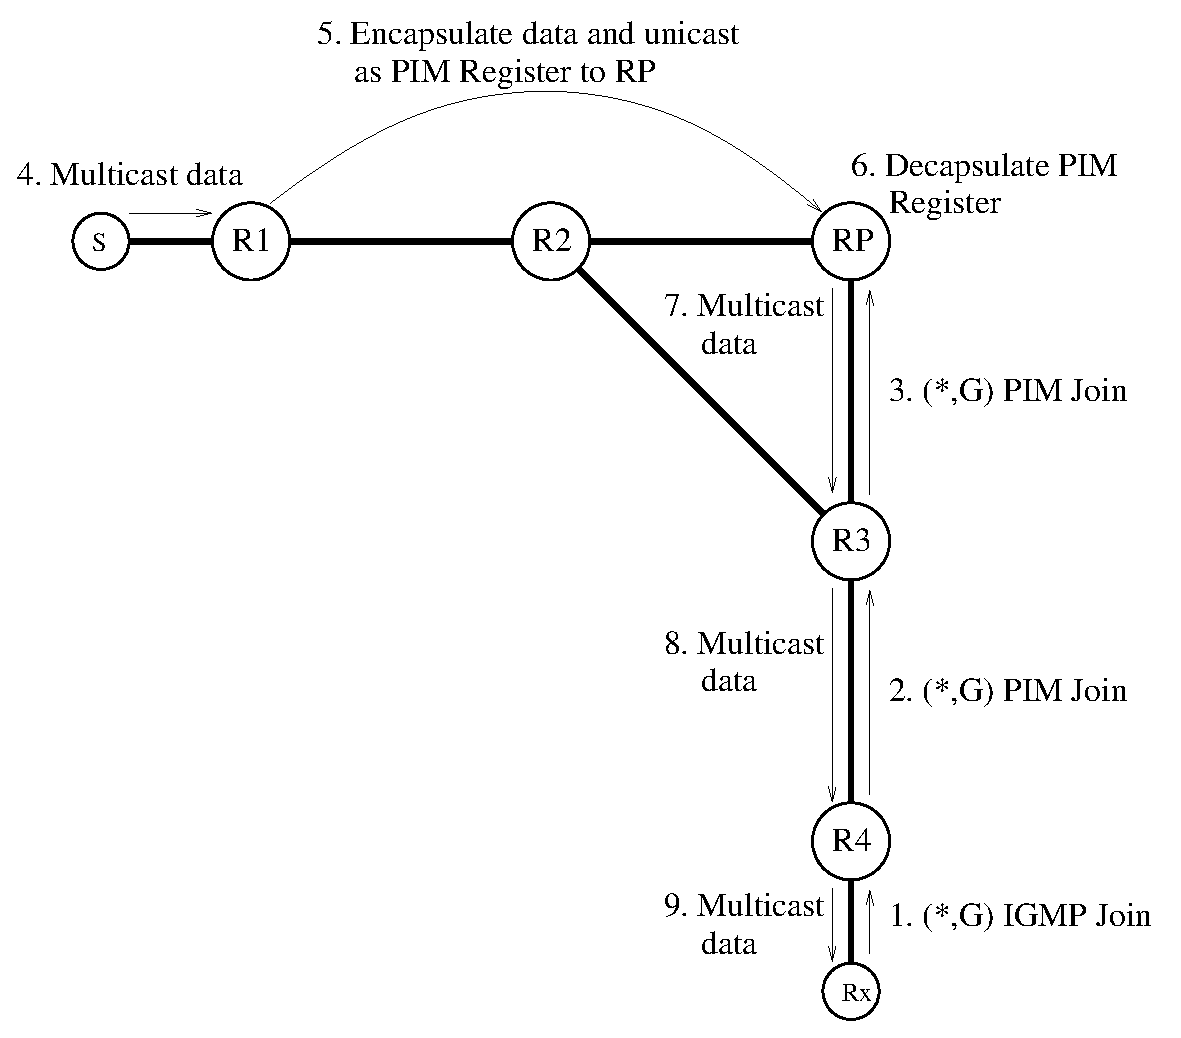
\includegraphics[width=6.0in]{figs/pim_protocol_overview1}
\end{center}

\end{slide}

%%======================================================================
\begin{slide}
\slidetitle{PIM-SM Example (cont.)}

\begin{center}
  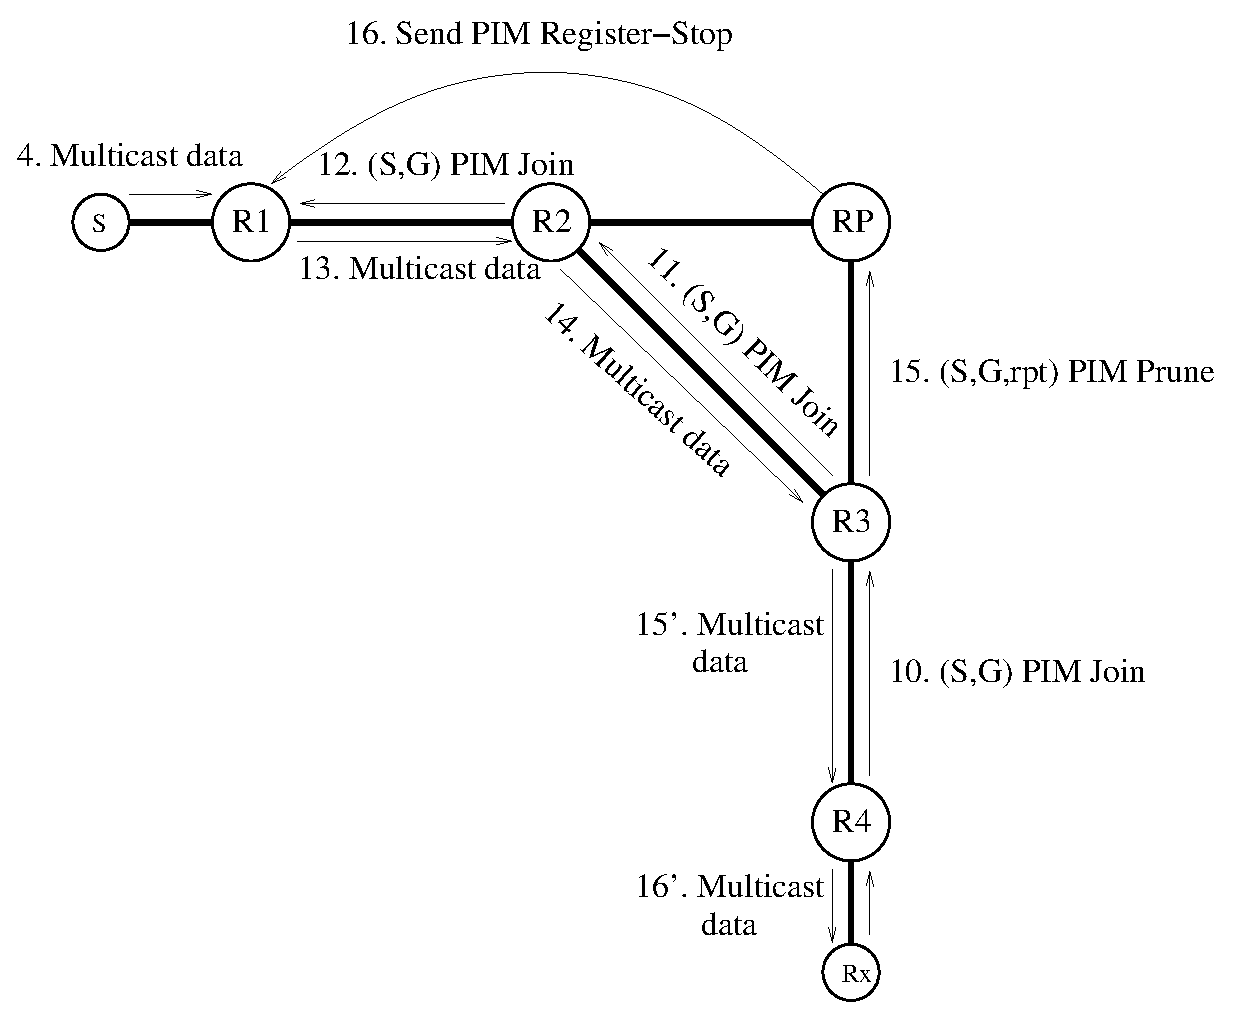
\includegraphics[width=6.0in]{figs/pim_protocol_overview2}
\end{center}

\end{slide}

%%======================================================================
\begin{slide}
\slidetitle{Xorp Architecture}

\begin{center}
  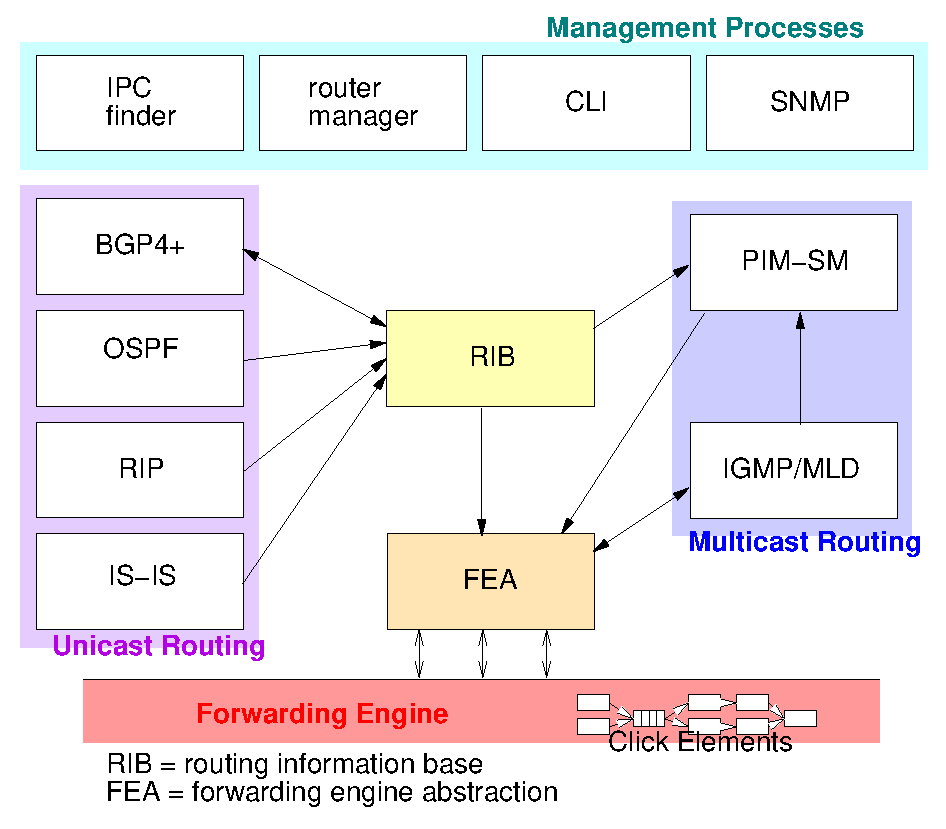
\includegraphics[width=6.0in]{figs/xorp_arch}
\end{center}

\end{slide}

%%======================================================================
\begin{slide}
\slidetitle{Interaction of Xorp PIM-SM with Other Modules}

\begin{center}
  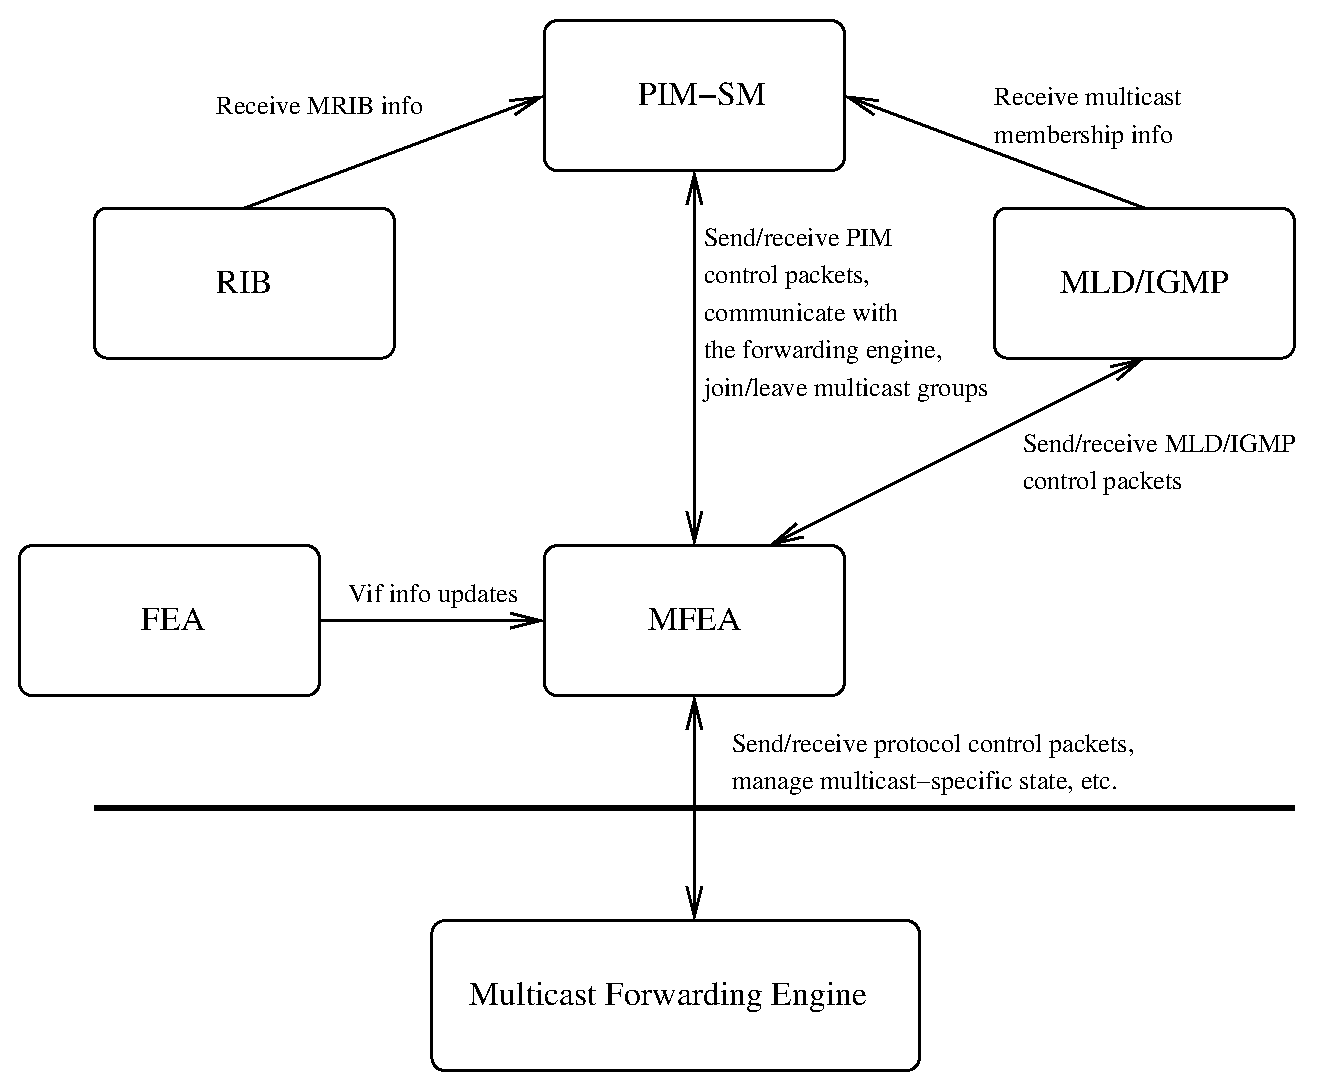
\includegraphics[width=6.0in]{figs/mcast_modules_interaction}
\end{center}

\end{slide}

%%======================================================================
\begin{slide}
\slidetitle{Xorp PIM-SM Abstraction}

\begin{center}
  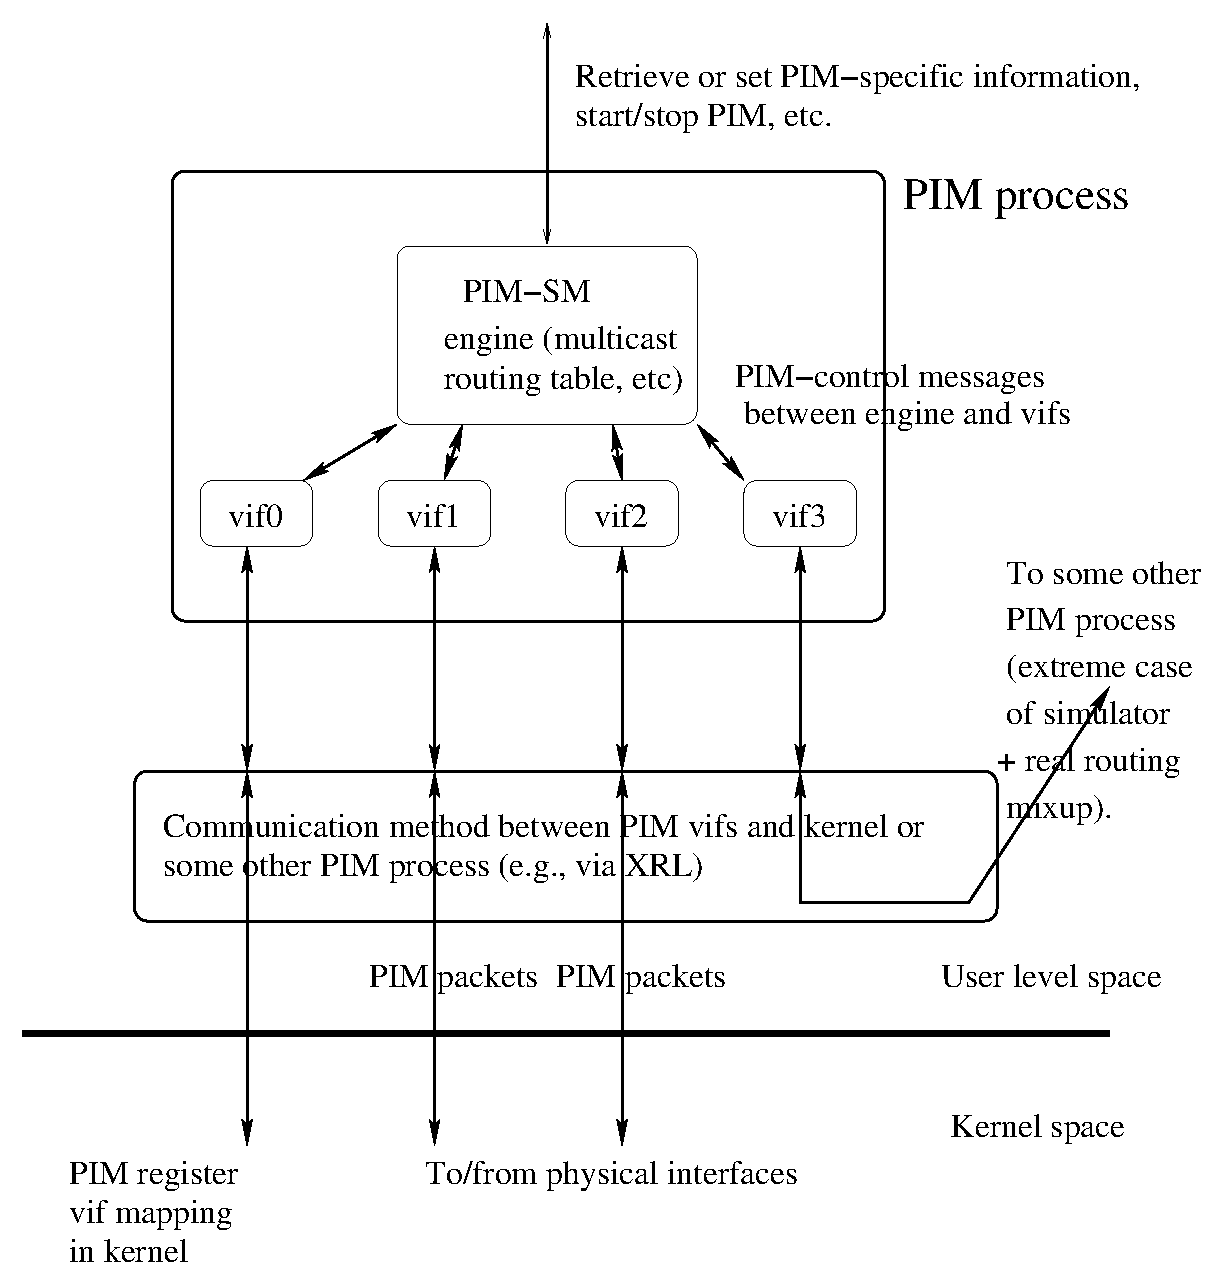
\includegraphics[width=5.5in]{figs/mcast_proto_abstraction}
\end{center}

\end{slide}

%%======================================================================
\begin{slide}
\slidetitle{Xorp PIM-SM Design Overview}

\begin{center}
  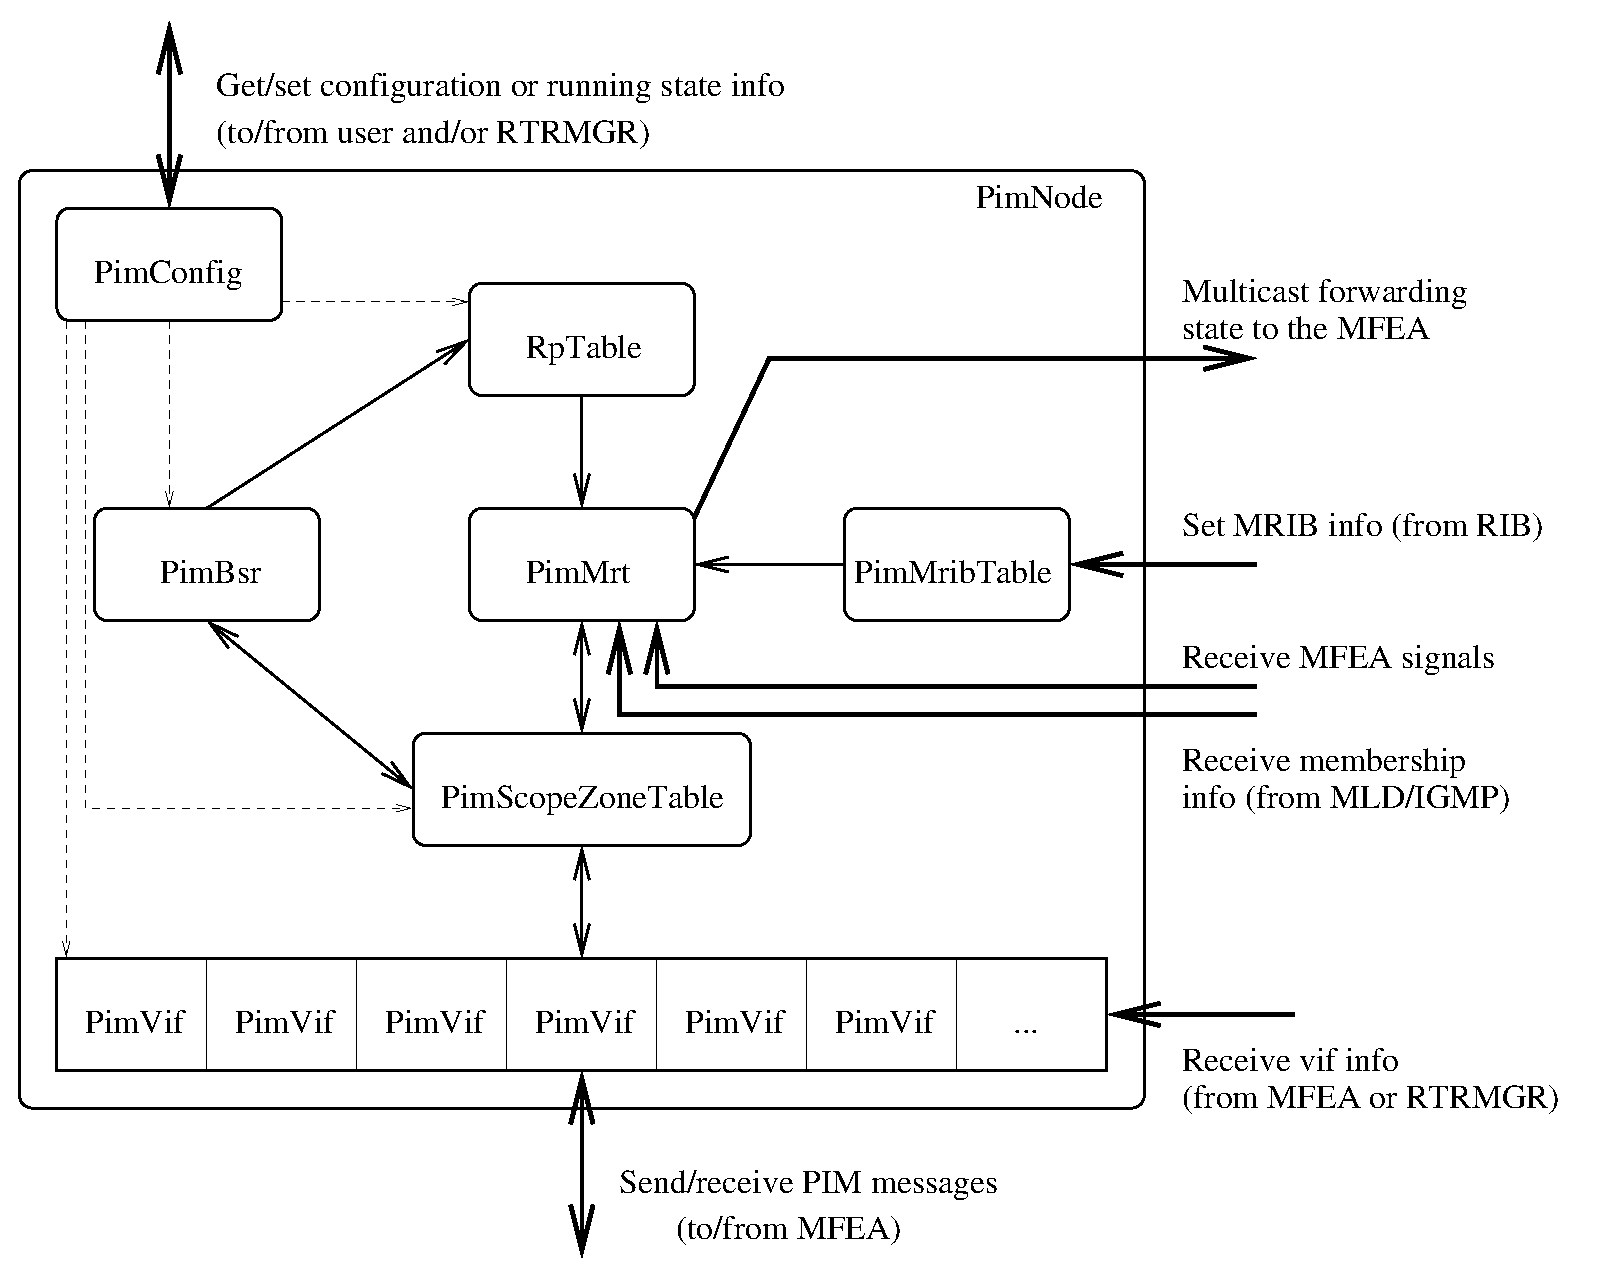
\includegraphics[width=6.0in]{figs/pim_design_overview}
\end{center}

\end{slide}

%%======================================================================
\begin{slide}
\slidetitle{Dependency Tracking Mechanism}

\begin{itemize}

  \item For each input event, what are the operations to perform and their
  ordering

  \item If the protocol is simple, you can take care of this by hand

  \item Unfortunately, this is not the case with PIM-SM:
  total of 52 input events, and 77 output operations.   

\end{itemize}

\end{slide}

%%======================================================================
\begin{slide}
\slidetitle{PIM-SM Dependency Tracking Mechanism}

PIM-SM spec has tens of macros like:

\begin{small}
\begin{verbatim}
pim_include(S,G) =
    { all interfaces I such that:
      ( (I_am_DR( I ) AND lost_assert(S,G,I) == FALSE )
        OR AssertWinner(S,G,I) == me )
       AND  local_receiver_include(S,G,I) }
\end{verbatim}
\end{small}

The corresponding state dependency rule is:
\begin{small}
\begin{verbatim}
void
PimMreTrackState::track_state_pim_include_sg(list<PimMreAction> action_list)
{
    track_state_i_am_dr(action_list);
    track_state_lost_assert_sg(action_list);
    track_state_assert_winner_sg(action_list);
    track_state_local_receiver_include_sg(action_list);
}
\end{verbatim}
\end{small}

\end{slide}

%%======================================================================
\begin{slide}
\slidetitle{Dependency Tracking}

\begin{center}
  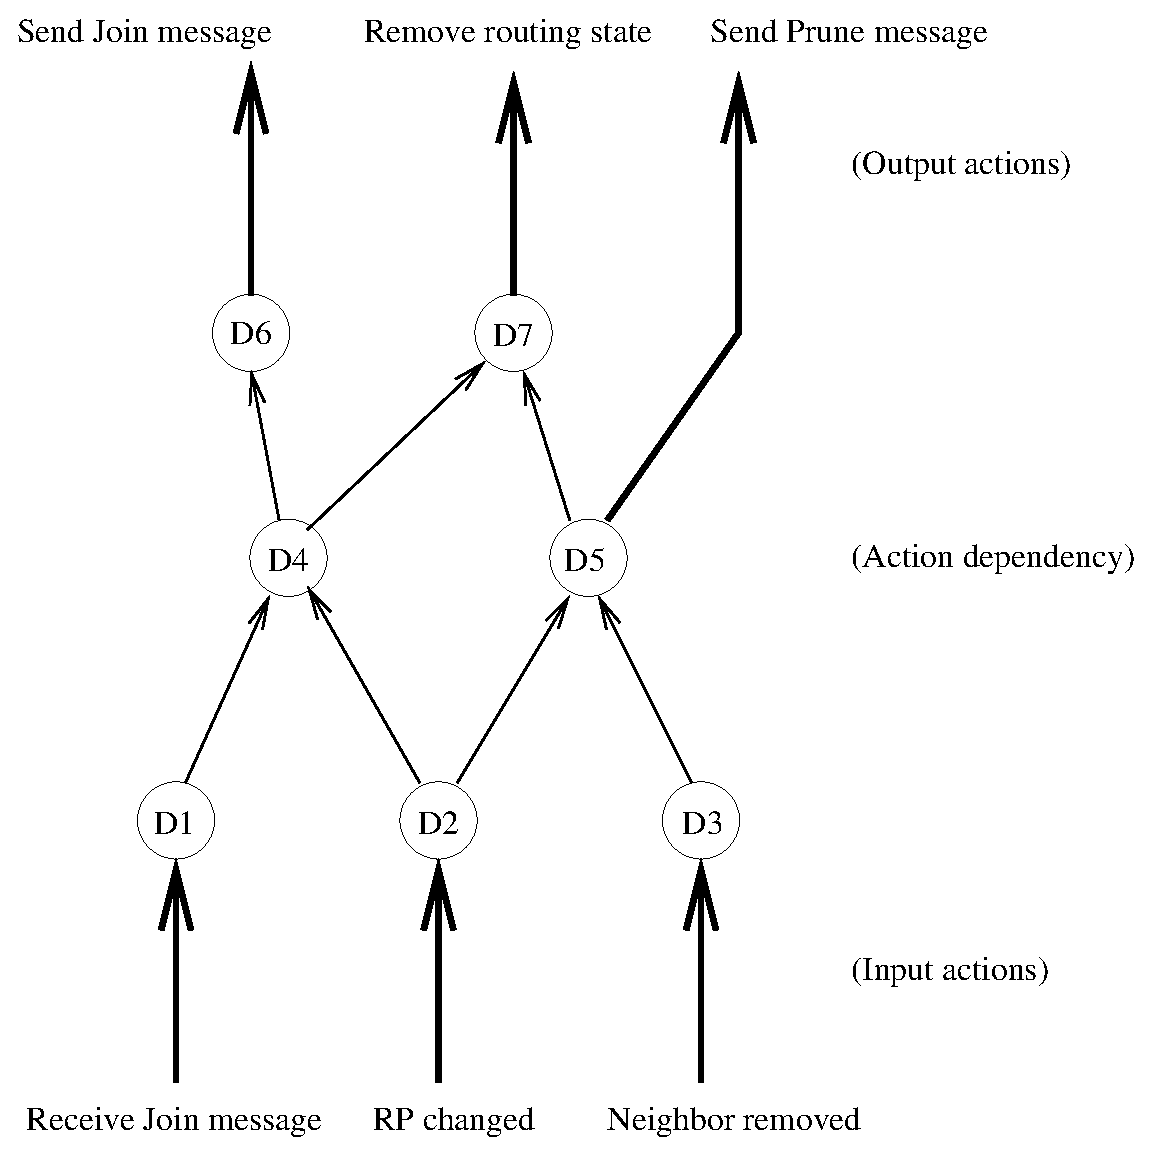
\includegraphics[scale=0.55]{figs/pim_state_dependency}
\end{center}

\end{slide}

%%======================================================================
\begin{slide}
\slidetitle{Dependency Tracking (2)}

\begin{center}
  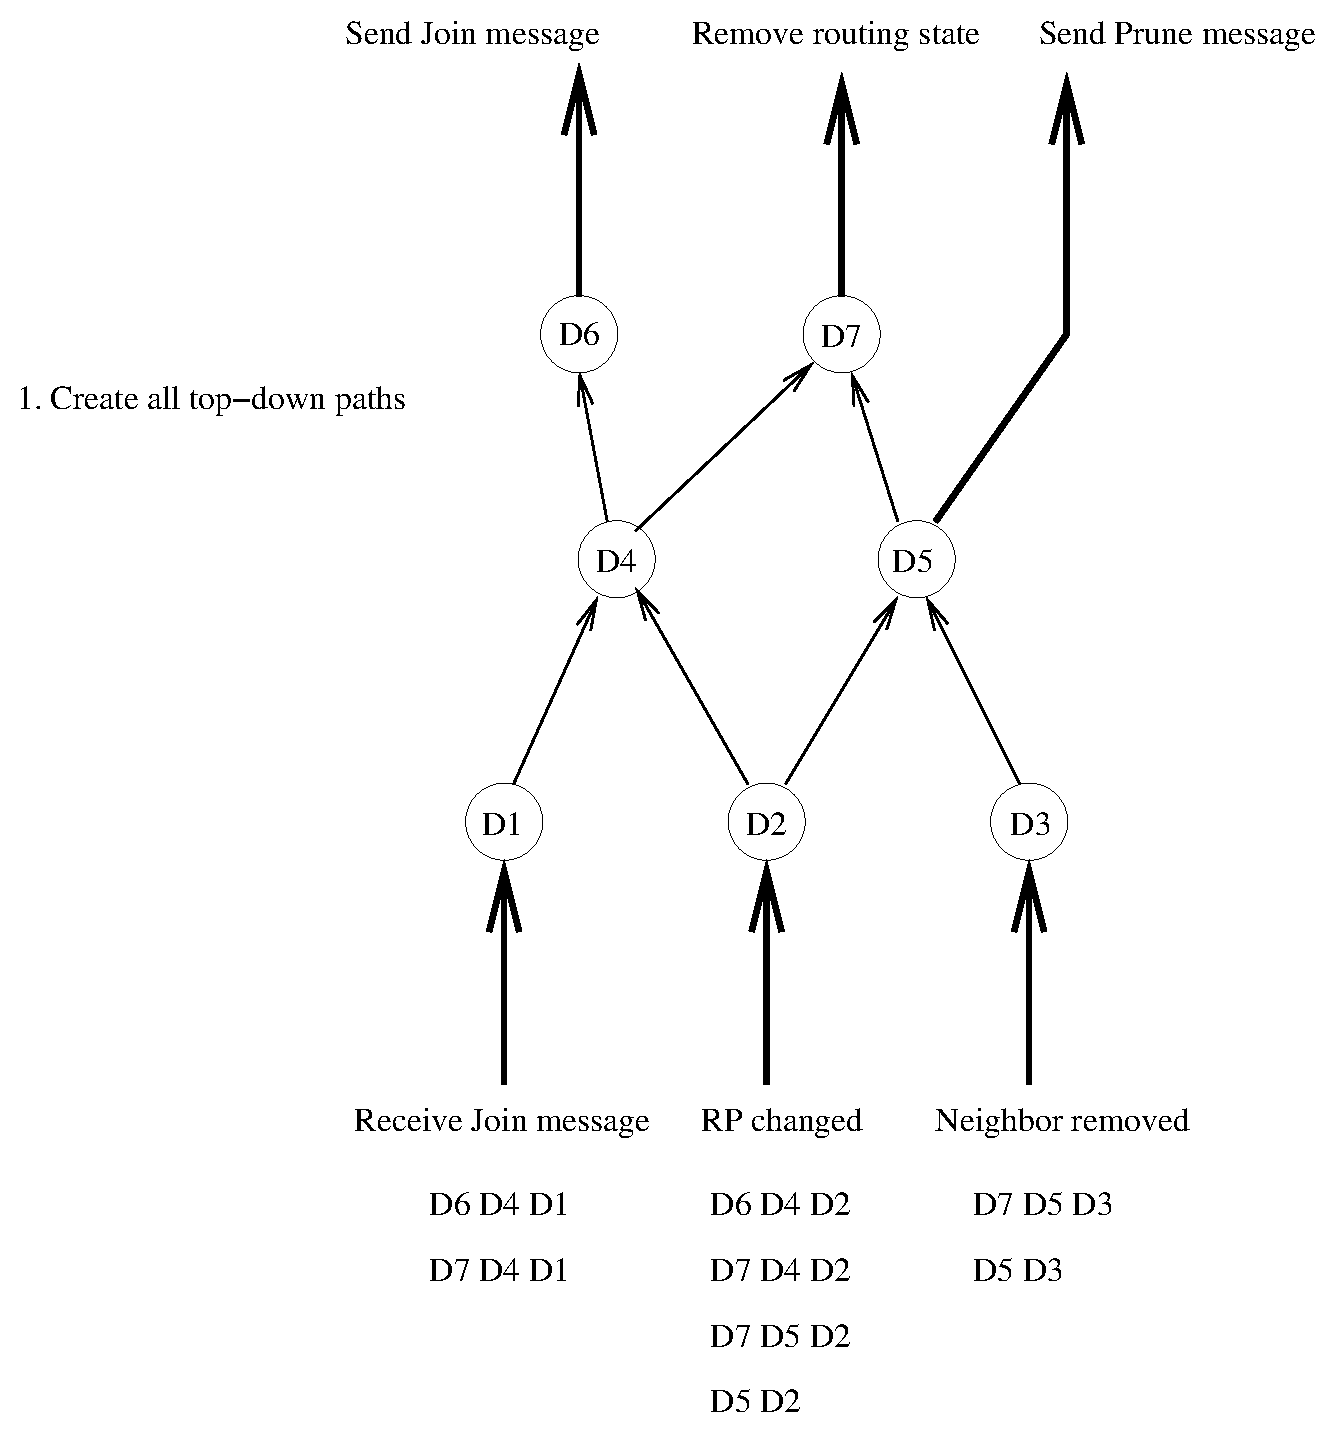
\includegraphics[scale=0.55]{figs/pim_state_dependency2}
\end{center}

\end{slide}

%%======================================================================
\begin{slide}
\slidetitle{Dependency Tracking (3)}

\begin{center}
  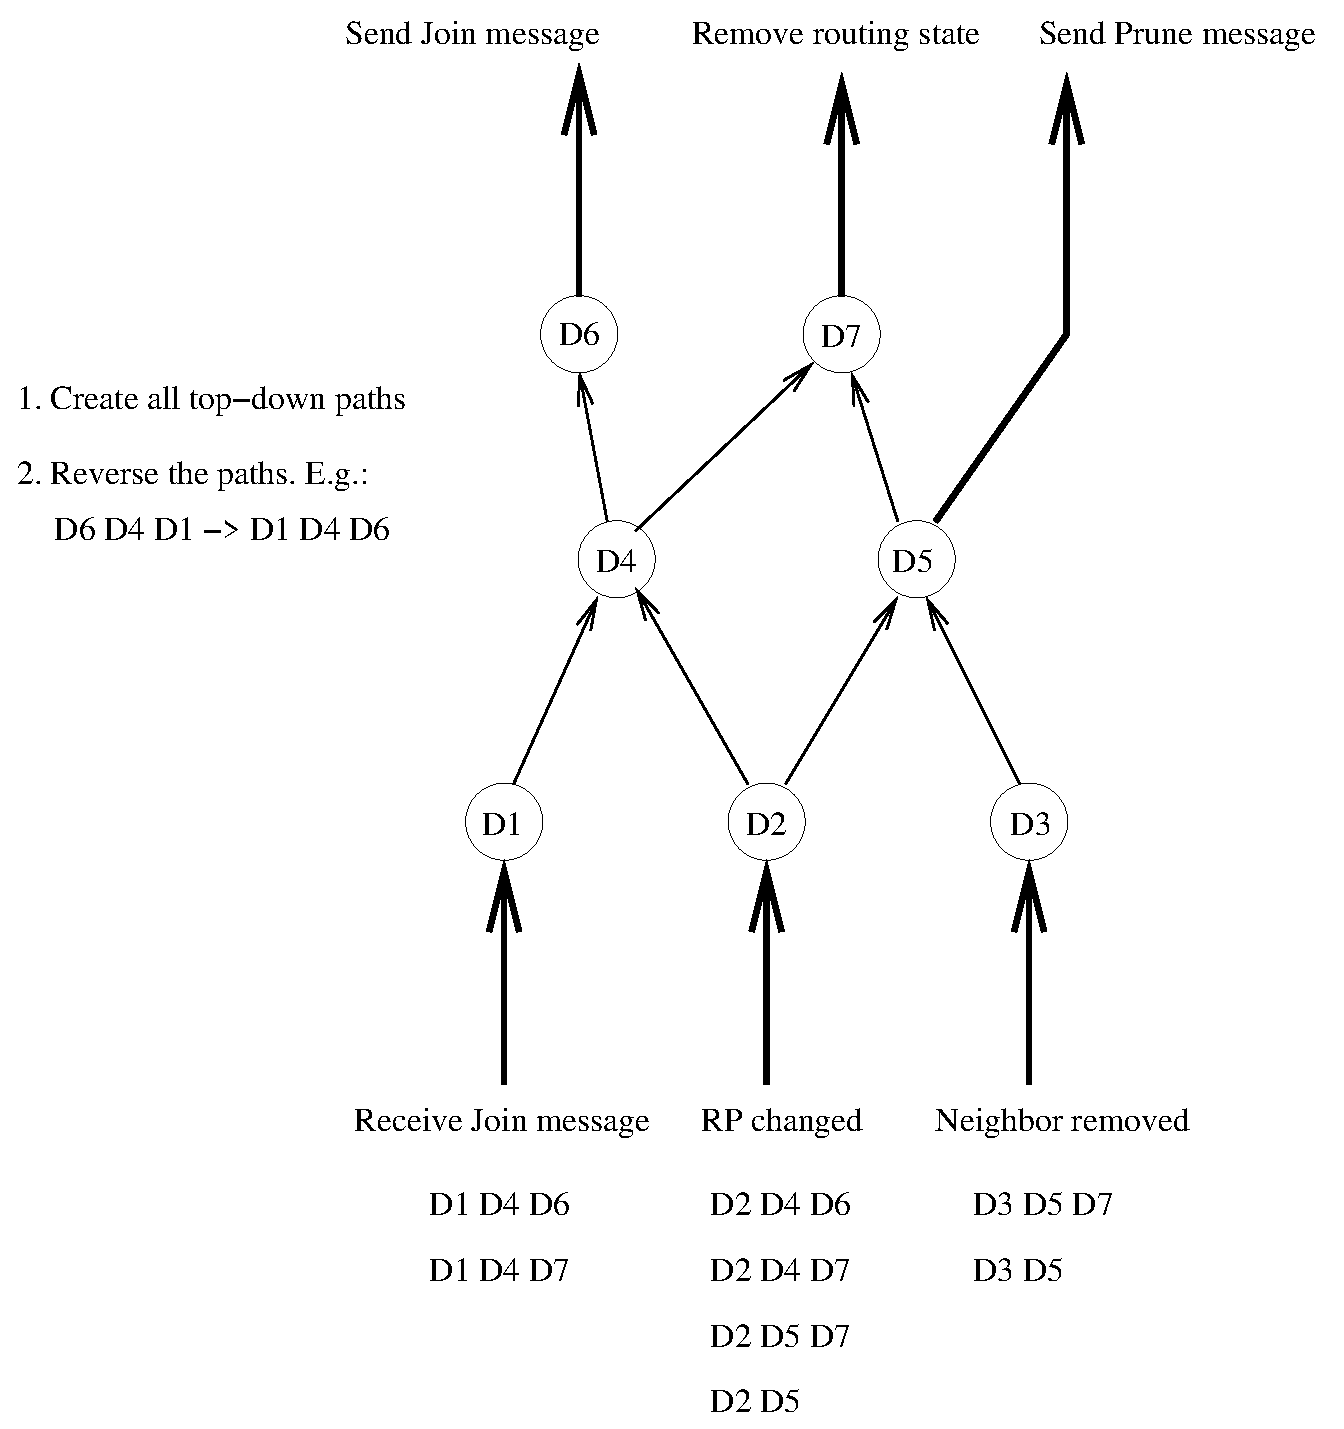
\includegraphics[scale=0.55]{figs/pim_state_dependency3}
\end{center}

\end{slide}

%%======================================================================
\begin{slide}
\slidetitle{Dependency Tracking (4)}

\begin{center}
  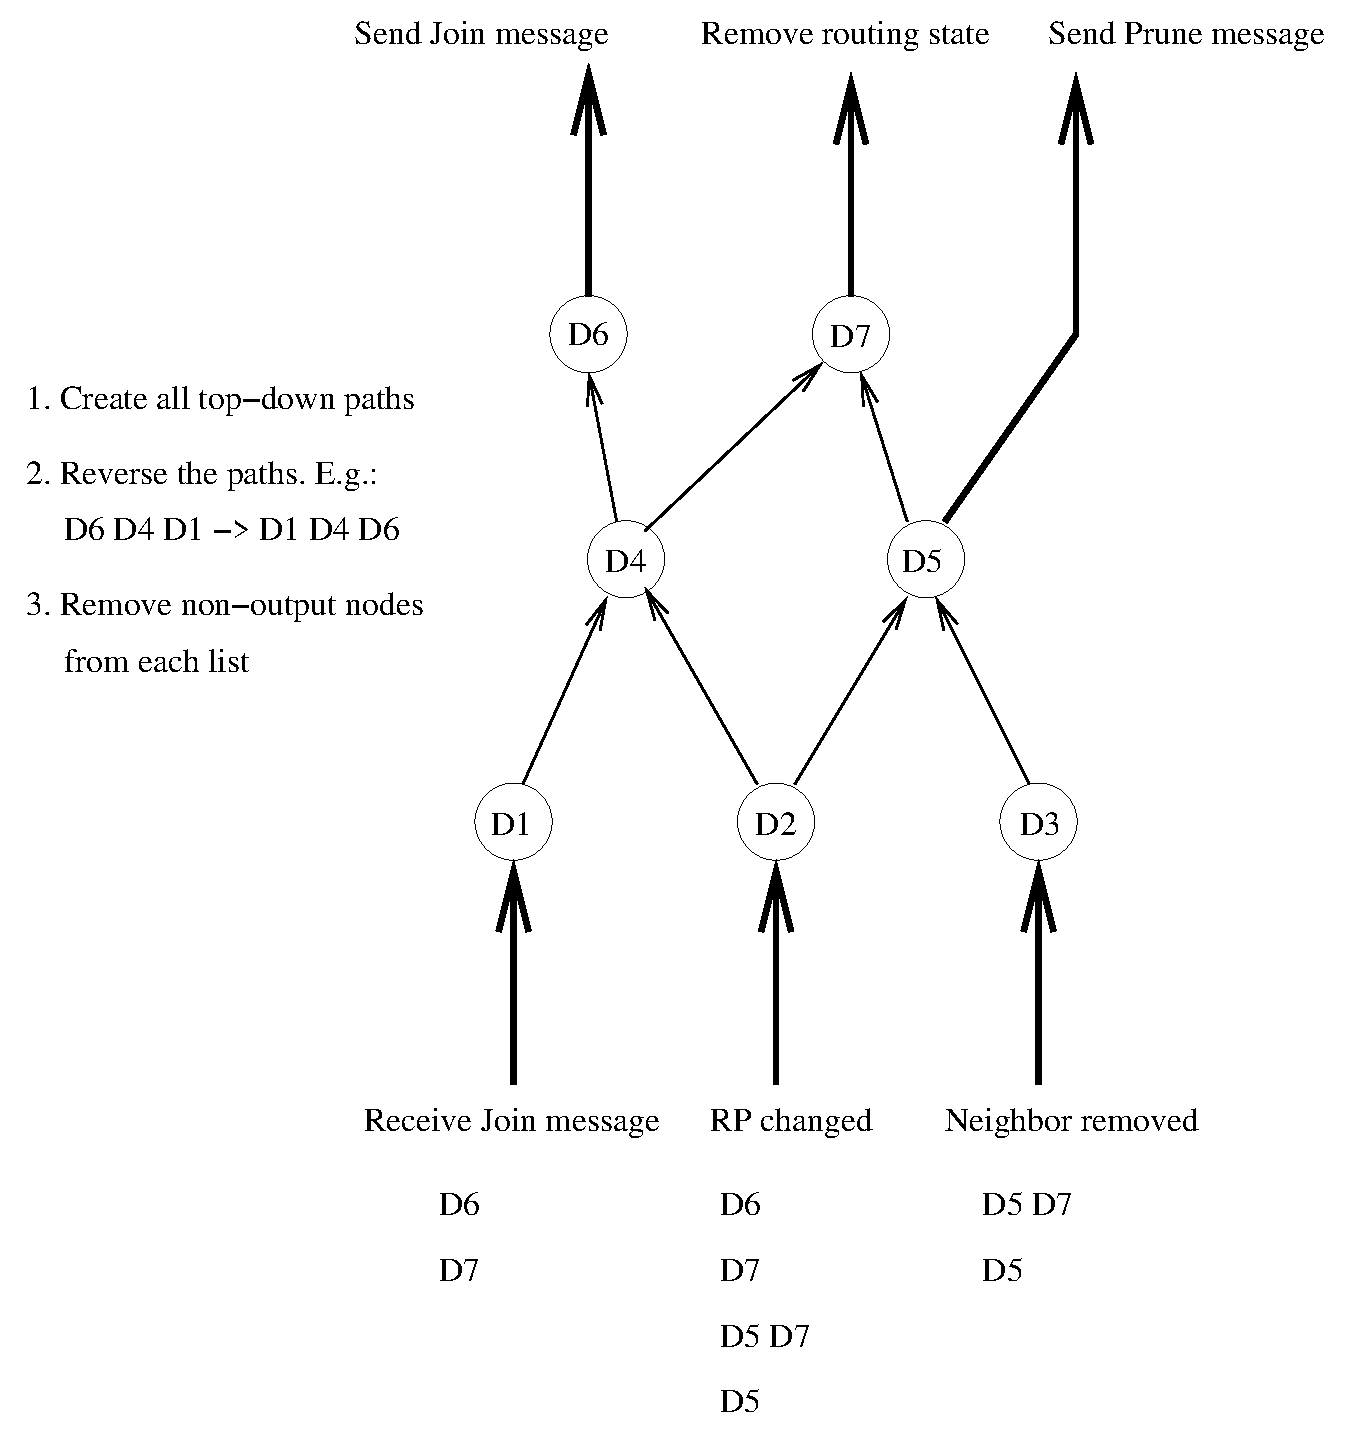
\includegraphics[scale=0.55]{figs/pim_state_dependency4}
\end{center}

\end{slide}

%%======================================================================
\begin{slide}
\slidetitle{Dependency Tracking (5)}

\begin{center}
  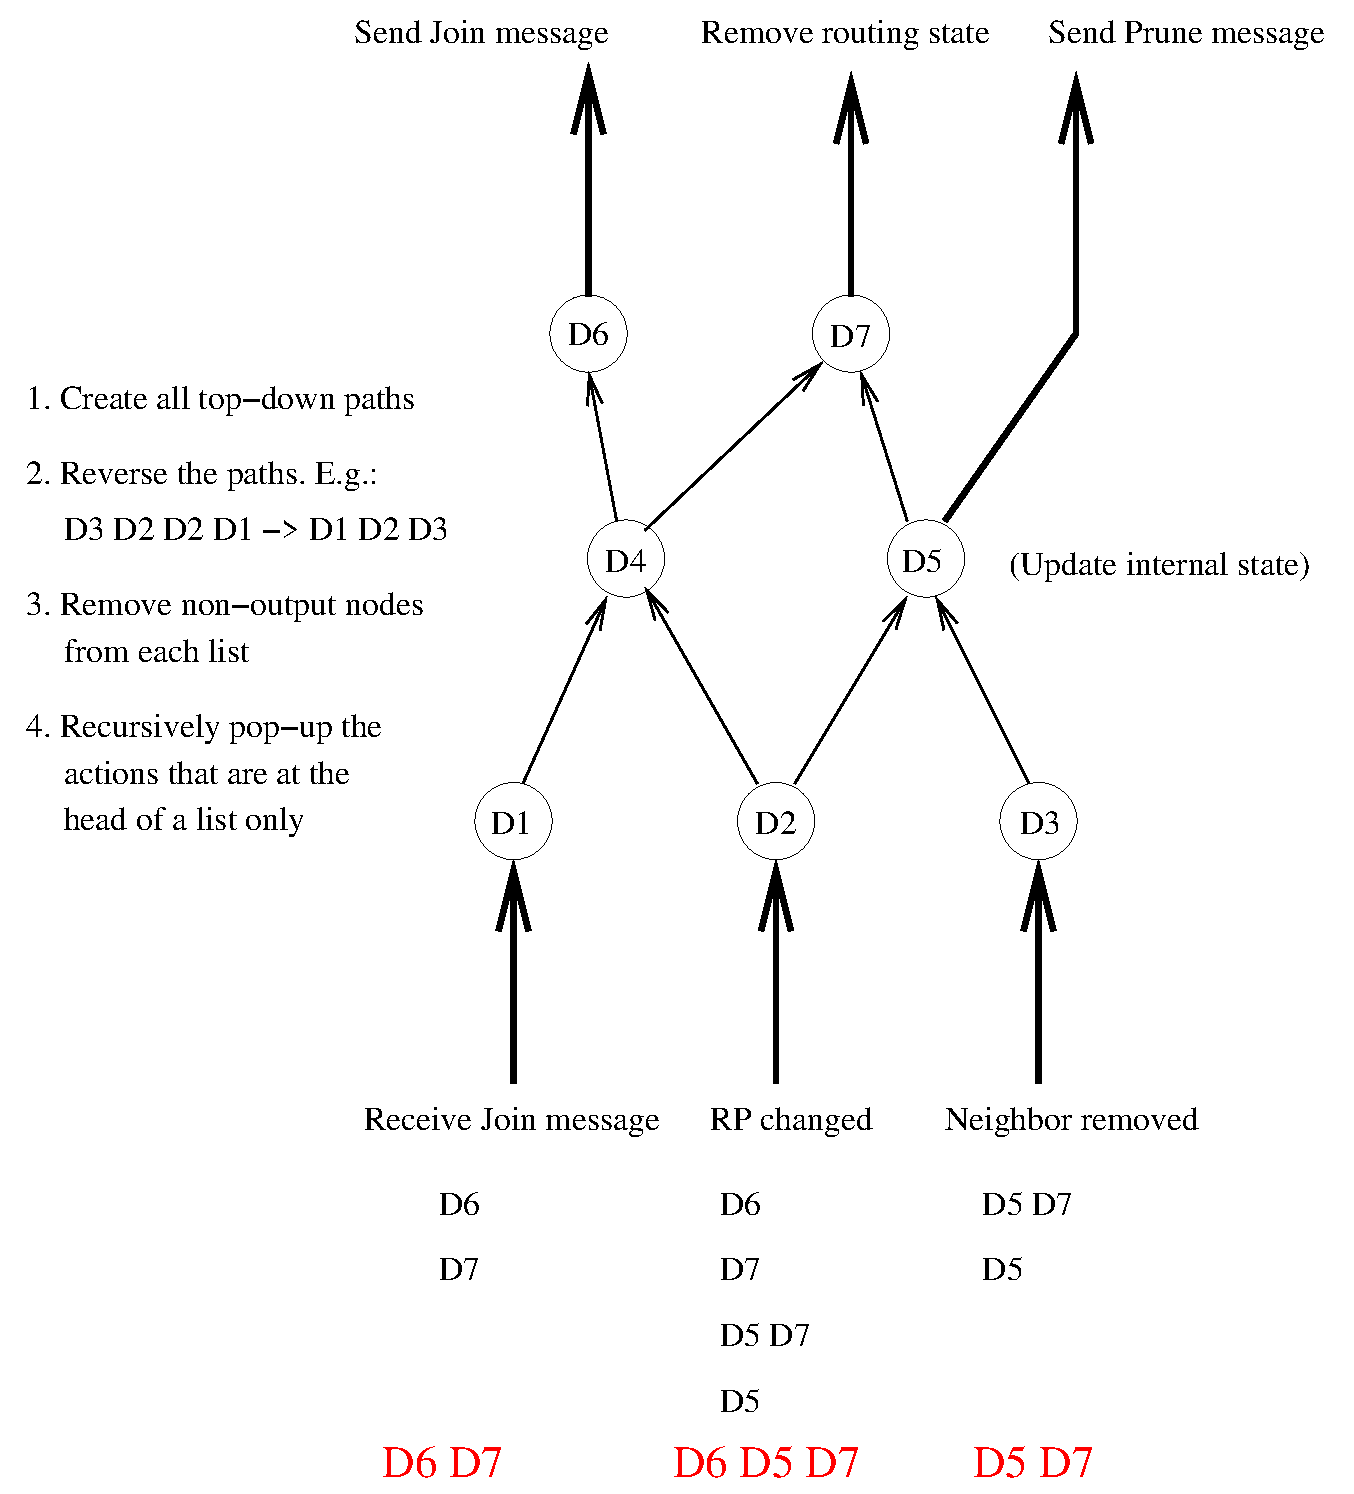
\includegraphics[scale=0.55]{figs/pim_state_dependency5}
\end{center}

\end{slide}

%%======================================================================
\begin{slide}
\slidetitle{Dependency Tracking Usage}

\begin{itemize}
  \item Each external event schedules (using FIFO) one or several tasks:
  \begin{itemize}
    \item Each task corresponds to an input event in the dependency tracking
    graph
    \item The list of actions associated with each task is taken from the
  dependency tracking graph
    \item A task may be applied to a number of routing entries (e.g., defined
  by an address prefix, RP address, neighbor address, etc.)
  \end{itemize}

\end{itemize}

\end{slide}

%%======================================================================
\begin{slide}
\slidetitle{Dependency Tracking Usage (cont.)}

\begin{itemize}
  \item A task is taken from the head of the queue, and is run to its
  completion, or until a pre-defined timeslot expires:
  \begin{itemize}
    \item If the timeslot expires, the remaining part of the task is
  added-back to the head of the queue
  \end{itemize}

  \item The time-slot computation prevents a huge task from blocking access
  to the process (e.g., if we want to perform emergency shutdown)
\end{itemize}

\end{slide}

%%======================================================================
\begin{slide}
\slidetitle{Dependency Tracking Summary}

\begin{itemize}
  \item The unidirectional ``graph'' is defined by the state computation
  macros

  \item For each macro, write the corresponding state dependency rule

  \item All state dependency is pre-computed on start-up

  \item If the spec changes, the rules are easy to update

  \item If the spec does not use macros for state computation, write your own
  macros

\end{itemize}

\end{slide}

%%======================================================================
\begin{slide}
\slidetitle{Status}

\begin{itemize}

  \item Completed: PIM-SM core (dual IPv4/v6), Bootstrap mechanism, Static RP,
  IGMPv1,2/MLDv1

  \item In progress: Integration with RIB, integration with RTRMGR

  \item Future work: IGMPv3/MLDv2, PIM-SSM, PIM-SM IPv6 testing,
  Bi-directional PIM

\end{itemize}

\end{slide}

%%======================================================================
\end{document}
